
\chapter{Foundations}
\label{ch:Foundations}
In this section we will present the \emph{Wiener process}. Then we show a way on how to discretize such a process in order to display it on a computer and to allow sampling from this stochastic process. 
We will show an algorithm which allows us to increase the number of time steps given a discretized sample path. This algorithm will be usefull for our numerical simulations.
In the last part of the chapter we will evaluate the \emph{stochastic integral} of a basic example using two distinct definitions. We will notice that the stochastic integral can be defined on many ways. In the next chapters we will focus on one particular defintion of the stochastic integral, namely the \emph{It\^o stochastic integral}.
\section{Stochastic processes}
\label{sec:}
\begin{samepage}
\begin{definition}[Stochastic process]
A stochastic process is a collection of random variables on a probability space \(\left( \Omega , \mathcal{F}, P\right)\)
indexed by time: 
\begin{displaymath}
\{X(t,\omega)\mid t\geq 0\}, \quad X(t,\omega)\!: [0,T]\times\Omega \rightarrow \mathbb{R}\;\;\text{for T given.}
\end{displaymath}
Measurability is meant to be w.r.t the product-\(sigma\)-algebra on \([0,T]\times\Omega\).
For each \(\omega \in \Omega\) we can define the mapping:
\begin{displaymath}
t\mapsto X(t,\omega)
\end{displaymath}
which we will call the \emph{sample path}, which is a realisation for a given \(\omega\). If this mapping is continuous, \(X_t\) is called a continuous stochastic process. 
\end{definition}
To simplify notation we will write \(X_t\) to denote a stochastic process on [0,T]. However notice that \(X_t\) is also a random variable for each t fixed.
\begin{definition}[Wiener process]
A Wiener process \(W_t\) (also called Brownian motion) is a continuous stochastic process satisfying:
\begin{enumerate}[noitemsep,topsep=0mm,labelindent=6mm,leftmargin=*,widest=3.,align=right]
\item \(W_0 = 0\) P-a.s
\item \(W_t-W_s \sim \mathcal{N}(0,t-s)\)
\item \(W_{t_1}-W_{s_1},\dots,W_{t_n}-W_{s_n}\) are independent for all non-overlapping intervals \([s_i, t_i],\: i=1,\dots,n\).
\end{enumerate}
\end{definition}
\nopagebreak
\begin{definition}[Adapted processes]
Let \(\mathcal{F}_t\) be the \(\sigma\)-algebra generated by \(\{W_s\mid 0\leq s\leq t\}\) for t\;\(\in[0,T]\). \(\mathcal{F}_t\) is called the \emph{filtration} induced by the Wiener process \(W_t\).
It holds that \(\mathcal{F}_s\subset\mathcal{F}_t\subset\mathcal{F}\) for \(s<t\), i.e. \(\{\mathcal{F}_t\}_{t\in[0,T]}\) is an increasing sequence of \(\sigma\)-algebras.
We will call a stochastic process \(X_t\) to be \(\mathcal{F}_t\)-adapted (or just adapted) if it is \(\mathcal{F}_t\)-measurable \(\forall\; t\in[0,T].\)\\
\emph{Take as example} \(X_t\coloneqq W_{t+1}\)\emph{, then }\(X_t\)\emph{ is not adapted.}
\end{definition}
\end{samepage}
\section{Discretization of the Wiener process}
Now We will consider the discretization of the Wiener process on [0,T] and we will denote it as \(\overline{W}_t\). We will use constant time steps only. Let \(\{t_0=0, t_1=\delta,\dots, t_n=n\delta\}\) be a time-grid with constant stepsize \(\delta\coloneqq\frac{T}{n}\).
\begin{algorithm}[Discretization of the Wiener process]
\begin{enumerate}[noitemsep,topsep=0mm,labelindent=6mm,leftmargin=*,widest=3.,align=right]
\item Initialize \(\overline{W}_0=0\)
\item For j = 0 to n-1
\begin{enumerate}[noitemsep,topsep=0mm,labelindent=6mm,leftmargin=*,widest=3.,align=right]
\item Generate z\(\sim \mathcal{N}(0,\delta)\)
\item Set \(\overline{W}_{(j+1)\delta} = z + \overline{W}_{j\delta}\)
\end{enumerate}
\item Linear interpolation to get a continious version.
\end{enumerate}
Then \((\overline{W}_0, \dots, \overline{W}_{n\delta}) \overset{d}{\sim} (W_0, \dots, W_{n\delta})\).
\end{algorithm}
We can indeed show that a process constructed this way is converging to the Wiener process as n goes to infinity.\footnote{This fact is known as Donsker's invariance principle or as functional central limit theorem. See for example \cite{Klenke}.} However the discretization itself is not a Wiener process since we lose the independence of the increments by using linear interpolation.
\begin{figure}[!h]
\centering
  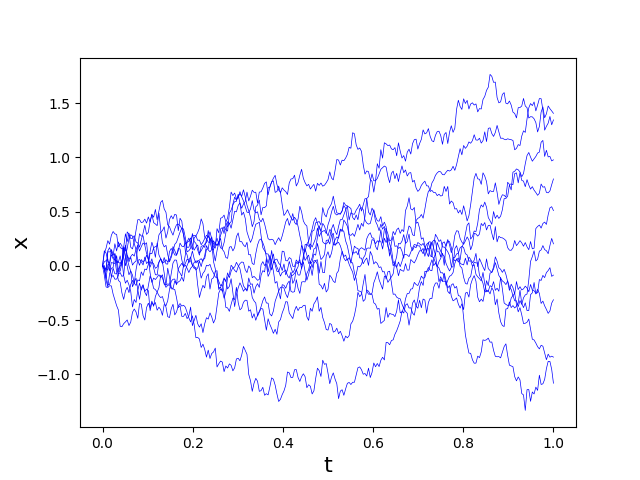
\includegraphics[scale=0.6]{content/Graphics/Figure_SamplingWienerProcess.png}
  \caption{10 realisations of discretizations of the Wiener process with n = 256 on [0,1].}
  \label{fig:fig1}
\nopagebreak
\end{figure}	

\begin{samepage}
To get a refinement for a given discrete sample path, we can use the following procedure. As an input we give a realisation of a discrete sample path \((\overline{W}_{t_0},\dots, \overline{W}_{t_n})\), n steps with step size \(\delta\). The output is a sample from the same process but with 2n steps: \(\left(\overline{W}_{R,t_0},\dots,\overline{W}_{R,t_n}\right)\), which makes a step size of \(\frac{\delta}{2}\).
We can use this procedure recursively to get finer and finer sample paths and imitate the convergence stated above.\footnote{See also Paul L\'evy's construction of the Wiener process in \cite{BMIntro} which follows the same idea.}
\begin{algorithm}[Refinement of a given discretized Wiener sample path]
\label{alg:Refinement}
\begin{enumerate}[noitemsep,topsep=0mm,labelindent=6mm,leftmargin=*,widest=3.,align=right]
\item For j = 0 to n-1
\begin{enumerate}[noitemsep,topsep=0mm,labelindent=6mm,leftmargin=*,widest=3.,align=right]
\item Generate \(z\sim \mathcal{N}(\frac{\overline{W}_{(j+1)\delta}+\overline{W}_{j\delta}}{2}, \frac{\delta}{4})\)
\item Set \(\overline{W}_{R,j\delta} = \overline{W}_{j\delta}\)
\item Set \(\overline{W}_{R,(j+\frac{1}{2})\delta} = z\)
\end{enumerate}
\item Set \(\overline{W}_{R,n\delta} = \overline{W}_{n\delta}\)
\item Linear interpolation.
\end{enumerate}
\end{algorithm}
This algorithm follows from the fact that \(W_{(j+\frac{1}{2})\delta}\mid_{ \!W_{j\delta}=a,\! W_{(j+1)\delta}\!=b} \sim \mathcal{N}({\frac{a+b}{2}}, \frac{\delta}{4})\).
\begin{figure}[!h]
\centering
  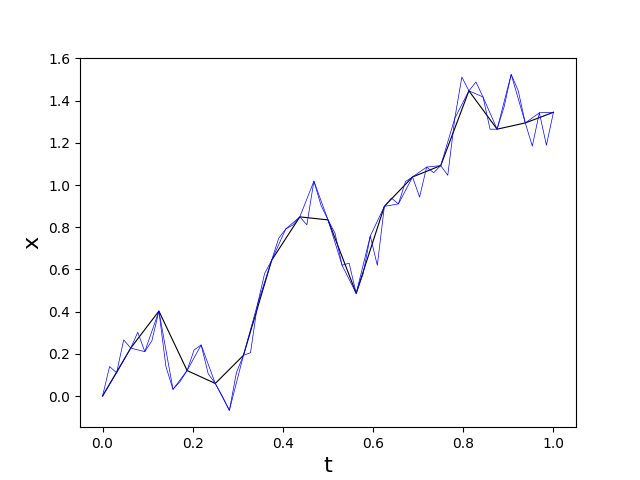
\includegraphics[scale=0.6]{content/Graphics/Figure_RefinementPath2.png}
  \caption{Finer versions of a given discretized Wiener process (black).}
  \label{fig:fig2}
\end{figure}
\end{samepage}
\section{Stochastic integration: It\^o and Stratonovich}
\label{sec:StochInt}
In this section we will present 2 (of many other possible) definitions of the stochastic integral for a basic example. We will show that both definitions yield different values.
Both definitions lead to 2 different stochastic calculii, the first one being called \emph{It\^o -} the second one \emph{Stratonovich stochastic calculus}.
In the next chapter (and in the rest of this thesis) we will focus on the definition due to It\^o and it will become clear, why this definition is more practical.


Our first attempt on defining the stochastic integral will be for the following example: 
\[\int_0^T \! 2W_t \, \mathrm{d}W_t.\]
The idea is to construct a partition of [0,T] and to evaluate the function only on these countable amount of time intervals, similar to Riemann(-Stieltjes)-sum approximation in the discrete case.
Then we take the limit of this sum and check for convergence in the \(L^2[\Omega]\)-norm.
Thus the stochastic integral will be defined as a limit of a sum of random variables and is thus also a random variable on the same probability space, if it exists\footnote{The limit of a sequence of measurable functions remains measurable, if it exists.}.
The limiting value will depend on which point on the intervals we evaluate the function. This is a counter-intuitive fact which does not hold in the deterministic case. If we evaluate the function at the start of each time interval, e.g. at \(t_j\) for \([t_j,t_{j+1}]\), we get the \emph{It\^o stochastic integral} and if we evaluate it at \(t_{j+\frac{1}{2}}\), at the middle of each time interval, we get the \emph{Stratonovich stochastic integral}.
\begin{definition}[Riemann-sum approximation]
Let \(P_n\) be a partition of [0,T], where n denotes the amount of steps. For our purposes we will consider only constant step sizes \(\delta\), e.g. \(P_n\coloneqq \{t_0 = 0, \dots, t_n = n\delta = T\}\) where T is fixed and \(\delta\) depends on n.
\begin{flalign*}
 R_{1,n} \coloneqq  R_1(P_n) &\coloneqq \sum_{k=0}^{n-1}2W_{t_k}\Delta W_{t_k}				  \tag{It\^o}  \\
 R_{2,n} \coloneqq  R_2(P_n) &\coloneqq \sum_{k=0}^{n-1}2W_{t_{k+\frac{1}{2}}}\Delta W_{t_k}   \tag{Stratonovich}
\end{flalign*}
where \(\Delta W_{t_k}\coloneqq W_{t_{k+1}}-W_{t_k}\) and \(W_{t_{k+\frac{1}{2}}}\) is the value of the process taken in the center of the interval [\(t_k, t_{k+1}\)].
\end{definition}
The key question which arises is whether \(R_{1,n}\) and \(R_{2,n}\) converge (in \(L^2[\Omega]\)) as n goes to infinity (e.g. \(\delta\) goes to 0). 
Indeed, using the proposition on quadratic variation which we will present later, we can show that the limits exist, but are not identical:
\begin{lemma}[Stochastic integration of \(\int_0^T \! 2W_t \, \mathrm{d}W_t\)]
\label{lemma:StochInt}
Let \(P_n\) be a partition of [0,T]. Then
\begin{flalign*}
 R_{1,n} &\rightarrow W_T^2 - T \quad  (\text{in } L^2[\Omega])\text{ as }n\to\infty \tag{It\^o} \\
 R_{2,n} &\rightarrow W_T^2 \quad       (\text{in } L^2[\Omega])\text{ as }n\to\infty \tag{Stratonovich}
\end{flalign*}
Notice also that \(W_T^2-T\) is a well-known martingale and \(W_T^2\) is what we would get in the deterministic case.
\end{lemma}
In order to calculate this, we need the following proposition:
\begin{proposition}[Quadratic variation]
Let \(P_n\) be a partition of [0,T]. Note that the step size \(\delta \rightarrow 0\) as \(n\rightarrow \infty\). Then
\[\sum^{n-1}_{k=0}(W_{t_{k+1}}-W_{t_{k}})^2 \rightarrow T \text{ as }n\rightarrow\infty\qquad(\text{in } L^2[\Omega]).\]
This implies the heuristic \((dW_t)^2=dt\) which is often seen in literature on stochastic calculus.
\end{proposition}
\begin{proof}
We will use the independence property of the Wiener process.
\begin{flalign*}
& \mathbb{E}[(\sum^{n-1}_{k=0}(W_{t_{k+1}}-W_{t_{k}})^2-T)^2] = \mathbb{E}[(\sum^{n-1}_{k=0}((W_{t_{k+1}}-W_{t_{k}})^2-\frac{T}{n}))^2]\\
& = \mathbb{E}[(\sum^{n-1}_{k=0}(x_k^2-\frac{T}{n}))^2] = \sum^{n-1}_{k,j=0}\mathbb{E}[(x_k^2-\frac{T}{n})(x_j^2-\frac{T}{n})]\\ 
& (\text{where }W_{t_{k+1}}-W_{t_{k}}\coloneqq x_k\sim\mathcal{N}(0,\frac{T}{n}))\\ 
& = \sum^{n-1}_{l=0}\mathbb{E}[(x_k^2-\frac{T}{n})^2] = \sum^{n-1}_{l=0}\text{Var}[x_k^2-\frac{T}{n}] + \underbrace{\mathbb{E}[x_k^2-\frac{T}{n}]^2}_{= 0}\\ 
& = \sum^{n-1}_{l=0}\textnormal{Var}[x_k^2] = 2n(\frac{T}{n})^2\rightarrow 0\text{ as }n\rightarrow\infty.
\end{flalign*}
\end{proof}
Now we are able to show lemma \ref{lemma:StochInt}.
\begin{proof}
We will show the lemma only for the It\^o-case:
\begin{flalign*}
& \mathbb{E}[(\sum^{n-1}_{k=0}2W_{t_{k}}(W_{t_{k+1}}-W_{t_{k}})-(W_T^2-T))^2] \\
& = \mathbb{E}[(\sum^{n-1}_{k=0}(W_{t_{k+1}}^2-W_{t_{k}}^2)-(W_{t_{k+1}}-W_{t_{k}})^2-(W_T^2-T))^2]\\
& (\text{Where we used that } 2X(Y-X) = (Y^2-X^2)-(X-Y)^2,\quad X\coloneqq W_{t_{k}}, Y\coloneqq W_{t_{k+1}})\\
& = \mathbb{E}[(\sum^{n-1}_{k=0}-(W_{t_{k+1}}-W_{t_{k}})^2+T)^2]\\
& = \mathbb{E}[(\sum^{n-1}_{k=0}(W_{t_{k+1}}-W_{t_{k}})^2-T)^2] \rightarrow 0, \text{ as }n\rightarrow\infty\ \\
& \text{using quadratic variation.}\quad\qquad
\end{flalign*}
\end{proof}
Is it possible to take other integrands than just \(2W_t\)?
In the next chapter we will give the idea behind the construction of the It\^o stochastic integral for a class of functions \(\mathcal{C}\) and we will give an argument on why we choose the definition of It\^o over the definition of Stratonovich.